\section{Fixed-point representation}
%
As a recall, when you are working on data with Python and Matlab, you generally deal with variables stored in the floating point representation as depicted in Fig.~(\ref{fig: 32}). This representation is close to what you learned as the \emph{scientific notation} and is convenient for simple operations as addition and multiplication.
%
\begin{figure}[H]
    \centering
    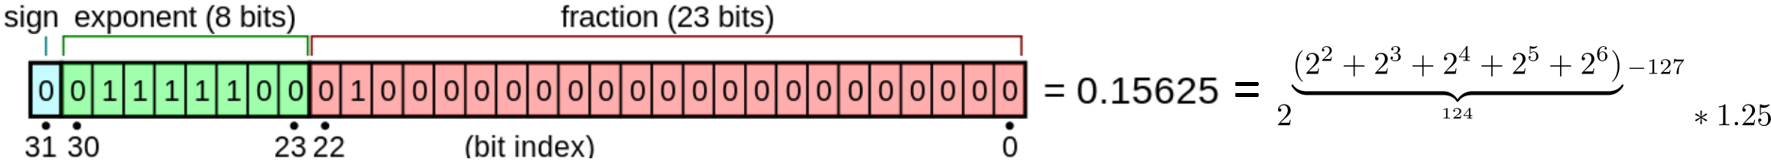
\includegraphics[width=\textwidth]{figs/Floating32.png}
    \caption{32-bit floating point example. The $1.0$ of $*1.25$ is implicit, meaning if all the fraction bits are $0$, we have $1.0$ by default}.
    \label{fig: 32}
\end{figure}
%
Unlike floating-point, the \emph{fixed-point} representation does not require 32 or 64 bits. This representation is closer to the binary format. The first bit is the \emph{sign} bit. Then we go from the Most Significant Bit (MSB) to the Least Significant Bit (LSB) by decreasing power of $2$. \\
Take the example of $8$-bit fixed-point. This means we can go in the range [$-128, 127$].
% A fixed-point representation does not give more than that, meaning we must store an implicit \emph{scaling factor} in memory to recover any initial value at the end. \\
% A way to see it is to always consider the signal is quantized in the range $\pm 1$ with a precision depending on the size of fixed-point representation. If you are measuring temperatures in the range $\pm 45$ [$\degree$C], this means you consider an implicit scaling factor of $45$ and you simply know:
% \begin{itemize}
%     \item $01111111 \rightarrow 1 \rightarrow 45$ [$\degree$C] is the maximum value.
%     \item $11111111 \rightarrow -1 \rightarrow -45$ [$\degree$C] is the minimum value (sign bit to 1)
%     \item $00000000 \rightarrow 0 \rightarrow 0$ [$\degree$C] is zero.
% \end{itemize}
%
\begin{bclogo}[couleur = gray!20, arrondi = 0.2, logo=\bcinfo]{Rescaling fixed points}
Think about multiplying your temperature signal by $8$, any value initially $>0.125$ will become larger than one and you will loose all the information about the signal. This is called \textbf{overflow}. In that case, you must first divide your signal by $8$ (equivalent to a $3$-bit shift to the right $\gg 3$).
% , and keep in mind your maximum value is now $45*8 = 360$ [$\degree$C].
This is called \textbf{rescaling} \\
\\
 In order to avoid overflows or precision loss, it often appears some functions rescale a signal in their computations. This information is given in the doc and you have to take it into account to recover the true amplitude of your final result. Note \emph{arm$\_$rfft$\_$q15} does rescale the signal, with a shift depending on the RFFT size, find the corresponding table in the doc.
\end{bclogo}
%
A practical example of an $8$-bit fixed-point signal is shown in Fig.~(\ref{fig: q4_4}). The default \textit{name} for such a signal is \emph{q1.7}. However, it is conventional to change this \textit{name} to keep track of the previous scalings. This is often critical when you convert a signal from fixed to float or inversely.
In this case, we have a \emph{q4.4} where we fixed the radix point.
% (keep in mind there is no practical difference).
%
\begin{figure}[H]
    \centering
    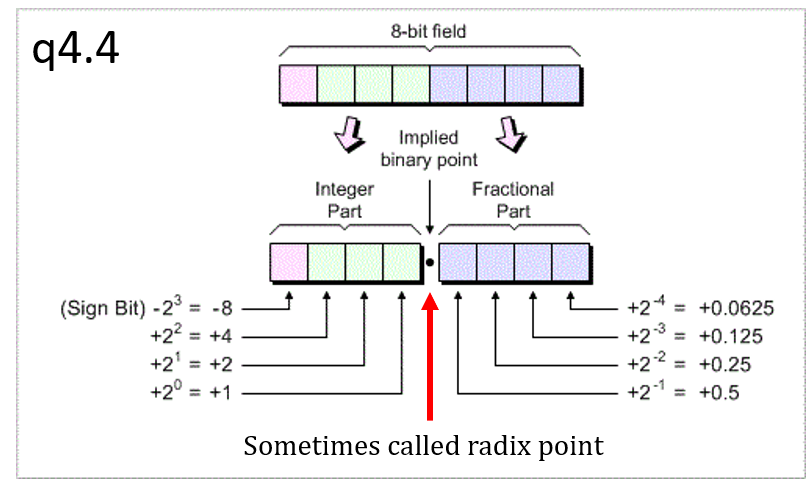
\includegraphics[width=10cm]{figs/fixed4_4.png}
    \caption{8-bit fixed point example \emph{q4.4}}
    \label{fig: q4_4}
\end{figure}
%
You can find a specific note of ARM on the fixed-point representation with pieces of code, named \emph{ARM$\_$fixed$\_$point}, in the \emph{Technical resources} directory on Moodle. \textbf{Read it carefully}, this is not wasted time. \\ \url{https://moodle.uclouvain.be/mod/folder/view.php?id=197742}. \\
Also find a description of the rules used by Matlab in practice for an FIR filter: \\ \begin{footnotesize}\url{https://fr.mathworks.com/help/dsp/ug/fixed-point-precision-rules-for-avoiding-overflow-in-fir-filters.html}\end{footnotesize}.
